% Fonte quantitativa desta seção:
% data/d4/resultados_d4_4.csv (rodadas), data/d4/resumo_celulas_d4_5.csv
% (células) e data/d4/contrastes_d4_5.csv (diferenças pareadas).
\section{D4 — Resultados e discussão}
\label{sec:resultados}

\subsection{Cenários e unidade de comparação}

A unidade de inferência foi uma janela operacional sintética de 8~h, iniciada com recursos livres
e filas vazias. Foram executadas 30 réplicas independentes, com 48 células por réplica: quatro
configurações de recursos sob as duas políticas da Tabela~\ref{tab:d4-desenho}, em cinco famílias
comuns, mais as células de agenda com informação perfeita. Dentro de uma réplica, todas as células
receberam os mesmos pedidos, manifestos, chegadas e durações. O piloto usou sementes distintas e
não foi combinado às rodadas definitivas. Cada efeito foi calculado primeiro dentro da réplica e
depois resumido pela média e pelo intervalo $t$ bilateral de 95\%, conforme o desenho de
comparações pareadas de \citet{law2023design}.

\begin{table}[htbp]
\centering\small
\caption{Configurações executadas. Cada contraste de infraestrutura alterou um recurso em relação
à Base. Todas as células mantiveram um TLOF, uma rota e uma estação de bagagem.}
\label{tab:d4-desenho}
\begin{tabular}{@{}lccccc@{}}
\toprule
Configuração & Stands & Balcões & Inspeções & FCFS local & Agenda \\
\midrule
Base & 5 & 1 & 1 & sim & sim \\
S4   & 4 & 1 & 1 & sim & sim \\
B2   & 5 & 2 & 1 & sim & sim \\
I2   & 5 & 1 & 2 & sim & sim \\
\bottomrule
\end{tabular}
\end{table}

A família de referência ofereceu 6 pedidos/h durante 7,25~h, com recarga de 30~min e observação
na janela completa. As sensibilidades usaram 4 e 8 pedidos/h, recarga de 0 e 60~min e informação
perfeita sobre chegadas e bagagem. A forma uniforme das chegadas continuou sendo hipótese do
cenário. Os indicadores principais foram definidos antes das rodadas: decolagens/h para política e
stands, espera média no balcão para B2 e espera média na inspeção para I2. Os demais indicadores
são descritivos ou exploratórios.

\subsection{Admissão, partidas e demanda atendida}

Na Base de referência, o FCFS produziu 4,221 decolagens/h (IC~95\%: 4,062--4,380), e a agenda,
4,092 (3,929--4,254). A diferença pareada agenda menos FCFS foi $-0,129$ decolagem/h
($-0,179$ a $-0,079$). A Figura~\ref{fig:d4-vazao-demanda} mostra que a diferença conservou o
mesmo sinal nas três taxas de demanda. As barras representam ICs de 95\% entre as 30 réplicas e
não a dispersão dos voos dentro de uma réplica.

\begin{figure}[htbp]
  \centering
  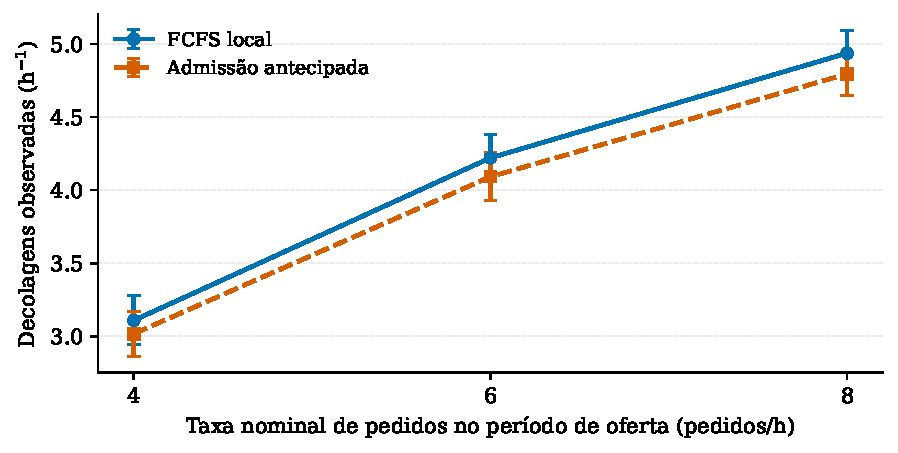
\includegraphics[width=0.92\linewidth]{figures/fig_d4_vazao_demanda.pdf}
  \caption{Decolagens observadas por hora na configuração-base, segundo a taxa nominal de pedidos
  durante o período de oferta. Pontos são médias de 30 réplicas independentes; barras são intervalos
  $t$ bilaterais de 95\%. FCFS e agenda compartilham o mesmo dia oferecido dentro da réplica.}
  \label{fig:d4-vazao-demanda}
\end{figure}

A Tabela~\ref{tab:d4-base-balanco} mantém o resultado de vazão ao lado da seleção de pedidos. Em
1.313 pedidos oferecidos nas 30 réplicas, a cobertura média foi 77,7\% sob FCFS e 75,4\% sob
agenda. O FCFS desviou em média 6,77 pedidos por réplica quando a chegada não começou na janela de
300~s; a agenda recusou 7,90 na decisão. Portanto, a menor espera observada entre passageiros
admitidos pela agenda não representa todos os pedidos oferecidos.

\begin{table}[htbp]
\centering\small
\caption{Balanço por réplica na Base de referência. Valores são média e IC~95\% entre 30
réplicas; a cobertura é decolados/pedidos oferecidos dentro de cada réplica.}
\label{tab:d4-base-balanco}
\begin{tabular}{@{}lcc@{}}
\toprule
Indicador & FCFS local & Agenda \\
\midrule
Pedidos oferecidos & 43,77 (41,48--46,05) & 43,77 (41,48--46,05) \\
Recusados & 0,00 (0,00--0,00) & 7,90 (6,63--9,17) \\
Desviados & 6,77 (5,67--7,87) & 0,00 (0,00--0,00) \\
Decolados & 33,77 (32,50--35,04) & 32,73 (31,43--34,03) \\
Pendentes no horizonte & 3,23 (2,66--3,80) & 3,13 (2,59--3,68) \\
Cobertura dos oferecidos & 77,7\% (75,5--80,0) & 75,4\% (73,0--77,7) \\
\bottomrule
\end{tabular}
\end{table}

A regra agendada manteve a saída planejada como horário mínimo. Depois de pronta para partir, a
aeronave reteve o stand por 75,9~s em média (IC~95\%: 70,1--81,7), contra 8,0~s
(6,3--9,6) no FCFS, embora a ocupação física média dos cinco stands fosse semelhante: 55,1\%
(53,0--57,2) e 55,3\% (53,2--57,4), respectivamente. Esse mecanismo é consistente com o sinal
negativo do contraste de política: a reserva antecipada reduziu admissões, mas o horário mínimo
também impediu algumas saídas antecipadas que ocorreriam no FCFS.

\subsection{Recursos, espera no terminal e retenção do grupo}

A Tabela~\ref{tab:d4-efeitos-principais} reúne os contrastes principais. O quinto stand acrescentou
cerca de 0,5 decolagem/h sob ambas as políticas. No S4, a média de desvios sob FCFS subiu de 6,77
para 11,27 pedidos por réplica, e a de recusas sob agenda, de 7,90 para 12,27. A ocupação física
por posição também aumentou de aproximadamente 55\% para 60\%. Assim, o contraste identifica
falta de posições no regime simulado, mecanismo compatível com o bloqueio de chegadas discutido
por \citet{onat2026buffer} e com os gargalos físicos distintos encontrados por
\citet{guerreiro2020}; não transfere para este cenário as capacidades numéricas desses estudos.

\begin{table}[htbp]
\centering\small
\caption{Contrastes principais na família de referência. Cada valor é a média das diferenças
dentro da réplica e seu IC~95\% ($n=30$). O sentido da subtração aparece na primeira coluna.}
\label{tab:d4-efeitos-principais}
\begin{tabular}{@{}llcc@{}}
\toprule
Contraste & Política & Efeito (IC~95\%) & Unidade \\
\midrule
Agenda $-$ FCFS, Base & --- & $-0,129$ ($-0,179$; $-0,079$) & decolagens/h \\
Base $-$ S4 & FCFS & 0,504 (0,453; 0,555) & decolagens/h \\
Base $-$ S4 & Agenda & 0,492 (0,440; 0,544) & decolagens/h \\
B2 $-$ Base & FCFS & $-141,5$ ($-158,4$; $-124,7$) & espera no balcão, s \\
B2 $-$ Base & Agenda & $-126,4$ ($-144,9$; $-107,9$) & espera no balcão, s \\
I2 $-$ Base & FCFS & 0,0 (0,0; 0,0) & espera na inspeção, s \\
I2 $-$ Base & Agenda & 0,0 (0,0; 0,0) & espera na inspeção, s \\
\bottomrule
\end{tabular}
\end{table}

O segundo balcão reduziu a espera média no balcão de 154,8 para 13,3~s sob FCFS e de 138,7
para 12,3~s sob agenda. Os denominadores foram 2.529 e 2.608 atendimentos sob FCFS na Base e em
B2, e 2.433 e 2.498 sob agenda. A fila não desapareceu do percurso: em B2, a espera média na
inspeção passou de zero para 8,0~s sob FCFS e 7,8~s sob agenda. O deslocamento para a estação
seguinte é coerente com a explicação de \citet{feldhoff2022}, que atribuiu a baixa espera na
inspeção ao atraso produzido no balcão. Como a Base já apresentou espera nula na inspeção nas 30
réplicas, o segundo posto de inspeção de I2 não tinha fila a remover; o zero da tabela é um
resultado observado no cenário, não uma afirmação de equivalência geral.

O alívio do balcão também antecipou a prontidão do grupo. Na Base, 9,2\% dos 987 voos FCFS
decolados com passageiros foram retidos pelo grupo, por 18,1~s em média; em B2, foram 2,3\% de
998 voos e 2,1~s. Sob agenda, as proporções foram 7,8\% de 957 voos na Base e 1,8\% de 960 em B2,
com retenções médias de 14,0 e 1,5~s. Essas reduções não produziram ganho comparável de vazão em
B2 porque, na família de referência, o ciclo do stand e a regra de admissão permaneceram mais
restritivos que a prontidão do pequeno conjunto de voos retidos.

\subsection{Sensibilidade, informação e alcance}

O contraste agenda menos FCFS na Base permaneceu negativo nas famílias de demanda baixa
($-0,092$ decolagem/h; IC~95\%: $-0,134$ a $-0,049$), demanda alta ($-0,142$;
$-0,189$ a $-0,095$), sem recarga ($-0,050$; $-0,084$ a $-0,016$) e recarga longa
($-0,083$; $-0,114$ a $-0,052$). Esses resultados são sensibilidades planejadas e não
comparações independentes de operações observadas.

Com recarga de 30~min, substituir as previsões declaradas por chegadas e bagagens realizadas
aumentou a vazão da agenda na Base em 0,092 decolagem/h (IC~95\%: 0,049--0,134). O aumento foi
0,083 no S4, 0,108 em B2 e 0,092 em I2. Sem recarga, o efeito na Base foi $-0,008$
decolagem/h ($-0,020$ a 0,004), e o intervalo incluiu zero. Portanto, neste desenho, a informação
perfeita compensou parte da reserva pessimista quando o ciclo incluiu 30~min de recarga, mas não
demonstrou ganho de vazão quando o stand era liberado rapidamente. Essa é uma comparação de
desenho informacional, não uma estimativa do valor econômico de dados operacionais.

Os resultados delimitam decisões do cenário: o quinto stand aumentou partidas; o segundo balcão
reduziu e deslocou espera; o segundo posto de inspeção foi redundante sob a carga que chegou a essa
estação; e a admissão antecipada, com horários mínimos e previsão pessimista, não superou o FCFS.
A interpretação não se estende a um vertiporto real. As durações são majoritariamente sintéticas,
a distribuição uniforme de chegada é suposta, cada stand tem carregador e gate próprios, a janela
começa vazia e as médias de espera incluem apenas visitas cujo atendimento começou. Recusas,
desvios, pendências e denominadores foram mantidos ao lado das médias para evitar confundir melhor
serviço entre admitidos com melhor atendimento da demanda oferecida. Os indicadores temporais são
medidas operacionais de nível de serviço; satisfação percebida exigiria declaração do passageiro e
não foi medida.
